\section{Modeling, Simulation, and Experimental Optimization Plan}

In order to create an experimental optimization plan for the project, first, the hardware and software constraints of the problem were identified. Since a different set of constraints can be applied based on the use-case, different models for each set of constraints were created. Finally, simulations were run on the generated models in order to analyze and understand what parts of the project to optimize through experimentation. The details of the code written for modeling and simulation can be found in Appendix \ref{sec:appendix-for-code}.

\begin{figure}[H]
    \centering
    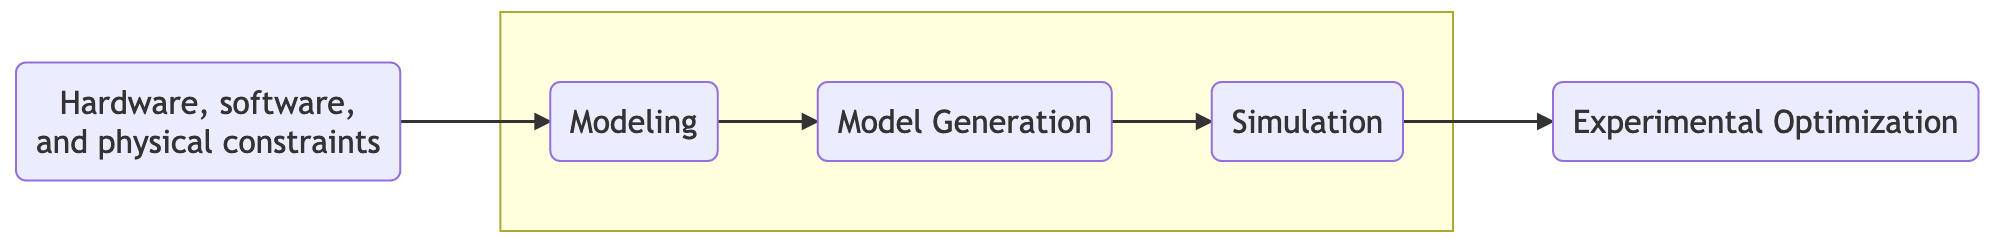
\includegraphics[width=0.95\textwidth]{final-proposal/images/mod_sim_flowchart.png}
    \caption{The high level flowchart capturing the modeling, simulation, and optimization process}
    \label{fig:mod-sim-flowchart}
% graph LR
%   model(Modeling)
%   modgen(Model Generation)
%   sim(Simulation)
%   opt(Experimental Optimization)
%   const(Hardware, software, <br> and physical constraints)

%   const --> model
%   subgraph " "
%     model --> modgen
%     modgen --> sim
%   end
%   sim --> opt
\end{figure}

%%%%%%%%%%%%%%%%%%%%%%%%%%%%%%%%%%%%%%%%%%
\subsection{Modeling}
The modeling was focused on hub-spoke and mesh networks. In each of the created models, each node represents the ESP8266 microcontroller-based physical devices, while the connections between the nodes represent the IEEE 802.11 based wireless communication. 

% Since the final design depends on the physical space, hardware, and software constraints of the project, the model was constructed with these constraints into consideration.%

According to our model, any two devices can only communicate if there is an established communication between them, and they are within each other's communication range. This models how wireless devices communicate with each other in the physical world. Given that the ESP8266 microcontrollers' built-in IEEE 802.11 based WiFi modules can typically connect with distances up to 100m \cite{chabukswardesign}, this is how we set the communication ranges for the nodes in our models.

Further, the number of simultaneous connections per device is also dependent on the hardware and software limitations. Since the ESP8266 microcontroller-based devices can have 8 simultaneous wireless connections \cite{ESP8266_NONOS_V1_1_0_Release_Notes}, the connection limit per node in our models follows this constraint as well.

Although using regular nodes is enough to create a mesh network, there need to be "hubs" in order to create a hub-spoke network topology. The hubs were modeled as special nodes that can handle a larger number of simultaneous connections in the network. It was also assumed that the hubs are connected to each other with low-latency and high-speed communication mediums, as is often the case in a typical home network where routers are connected in this manner. 

In using the aforementioned "nodes" and "hubs", different network models were generated to represent various real-life network conditions. The next subsection explains how these models are generated.


%%%%%%%%%%%%%%%%%%%%%%%%%%%%%%%%%%%%%%%%%%
\newpage
\subsection{Model Generation}
\label{model-gen-section}
First, a two-dimensional rectangular virtual space was created based on the physical space constraints. The virtual space was configured to be flexible in terms of dimensions to accommodate different physical space requirements. Later, the target number of nodes were placed into the virtual space randomly using Python's \cc{randint()} method in order to prevent possible biases, as shown in \ref{fig:modeling_node}.

\begin{figure}[H]
    \centering
    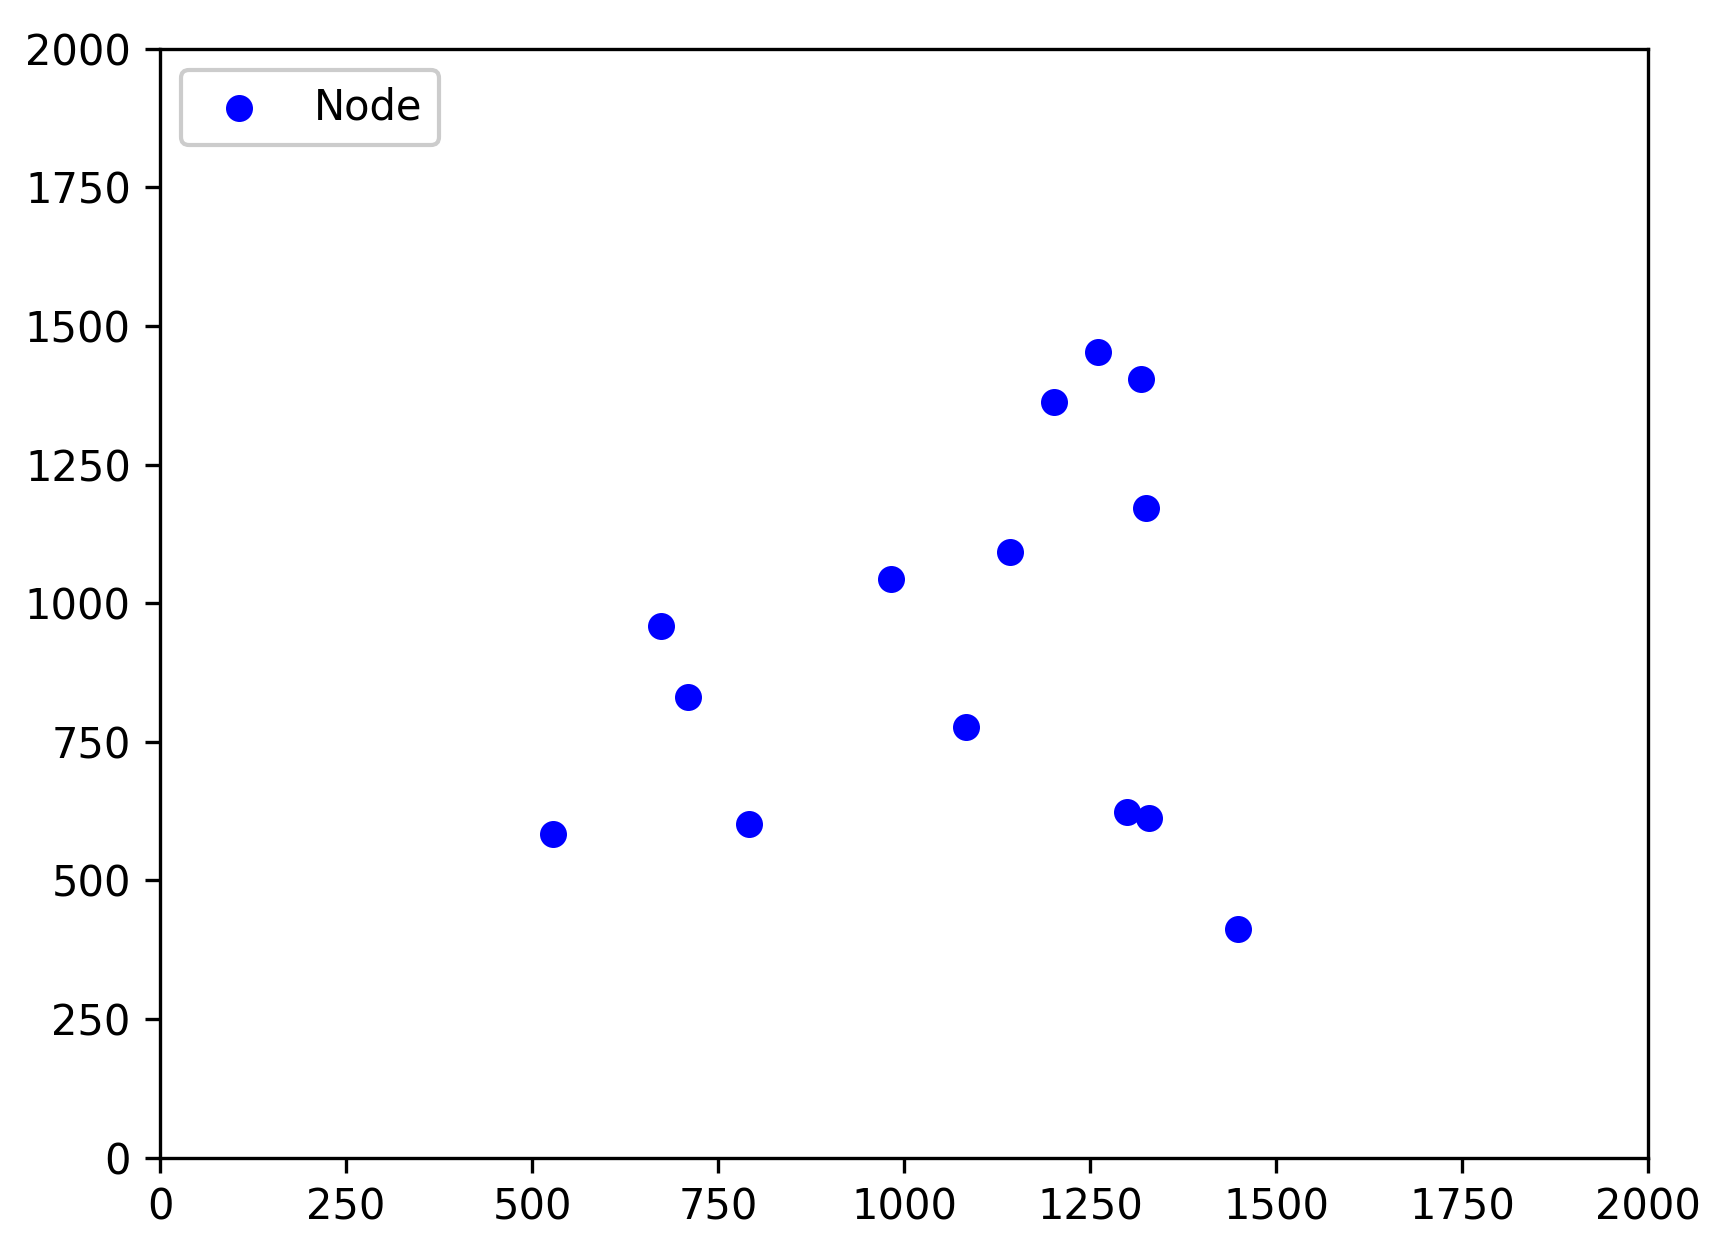
\includegraphics[width=0.5\columnwidth]{final-proposal/images/modeling_nodes_only.png}
    \caption{Nodes randomly distributed in the virtual space}
    \label{fig:modeling_node}
\end{figure}


Once the placement was completed in Figure \ref{fig:modeling_node}, the communication range of each node was determined within the virtual space, as shown in Figure \ref{fig:modeling_mesh}. Based on the simultaneous connection budget available for each node and overlapping communication ranges, the connections between the nodes can be created to construct a mesh network, as shown in Figure \ref{fig:modeling_mesh}.

\begin{figure}[H]
    \centering
    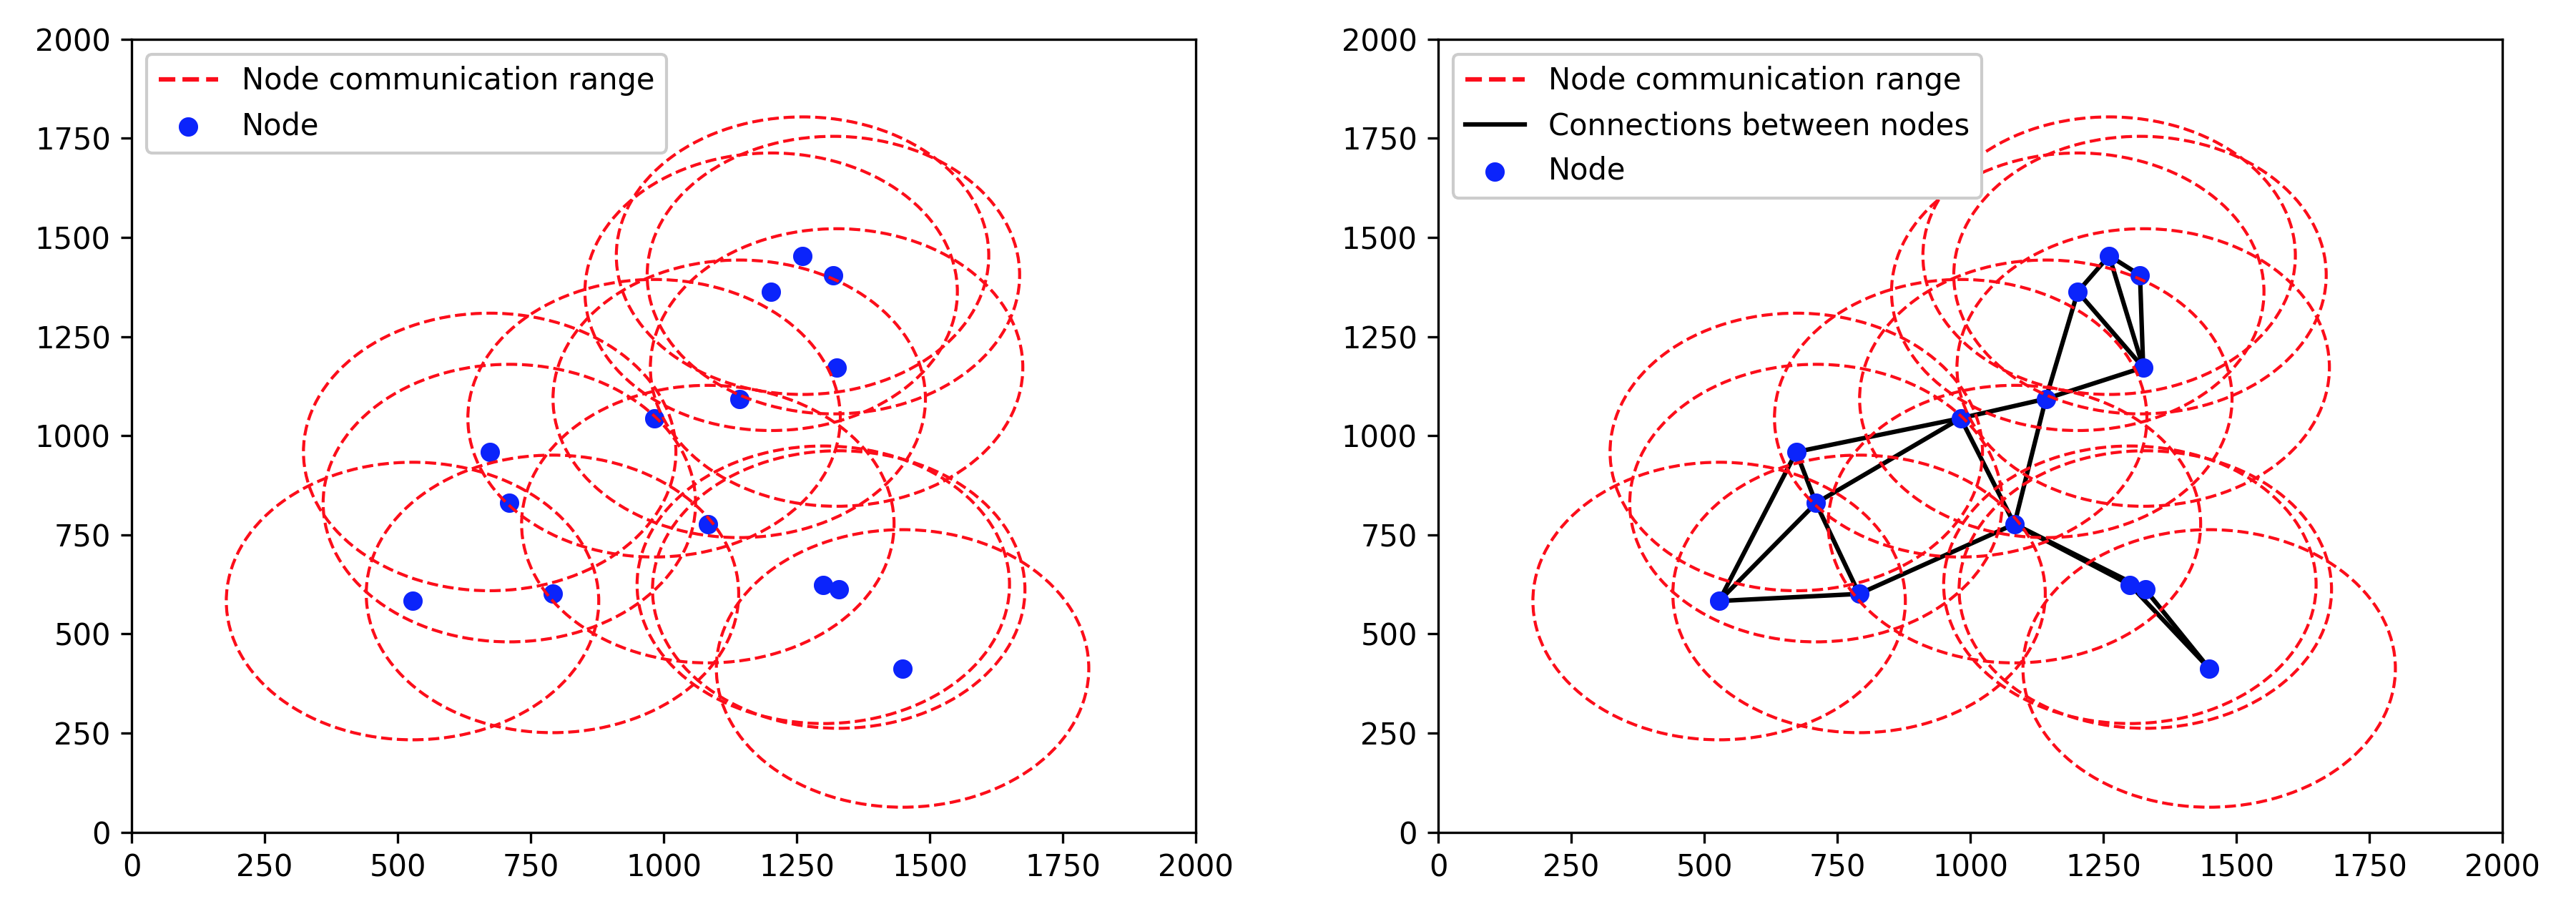
\includegraphics[width=0.94\columnwidth]{final-proposal/images/modeling_mesh.png}
    \caption{Left: Nodes and their communication ranges, Right: Nodes connected in mesh network topology based on the communication ranges}
    \label{fig:modeling_mesh}
\end{figure}

A hub-spoke network was also created from the random node placement shown in Figure \ref{fig:modeling_node}. However, it is not enough to simply check for the connection budget and overlapping communication ranges to construct a hub-spoke network topology, as was done for the mesh network. The nodes must communicate with each other via hubs. In order to find the optimal placement of the hubs for the created network, the "k-means" algorithm was applied iteratively until the created group of nodes covered the entire network. Next, a hub was placed at the center of each group, as shown on the left in Figure \ref{fig:modeling_star}. Nodes were then connected to the hubs, as shown on the right in Figure \ref{fig:modeling_star}.

\begin{figure}[H]
    \centering
    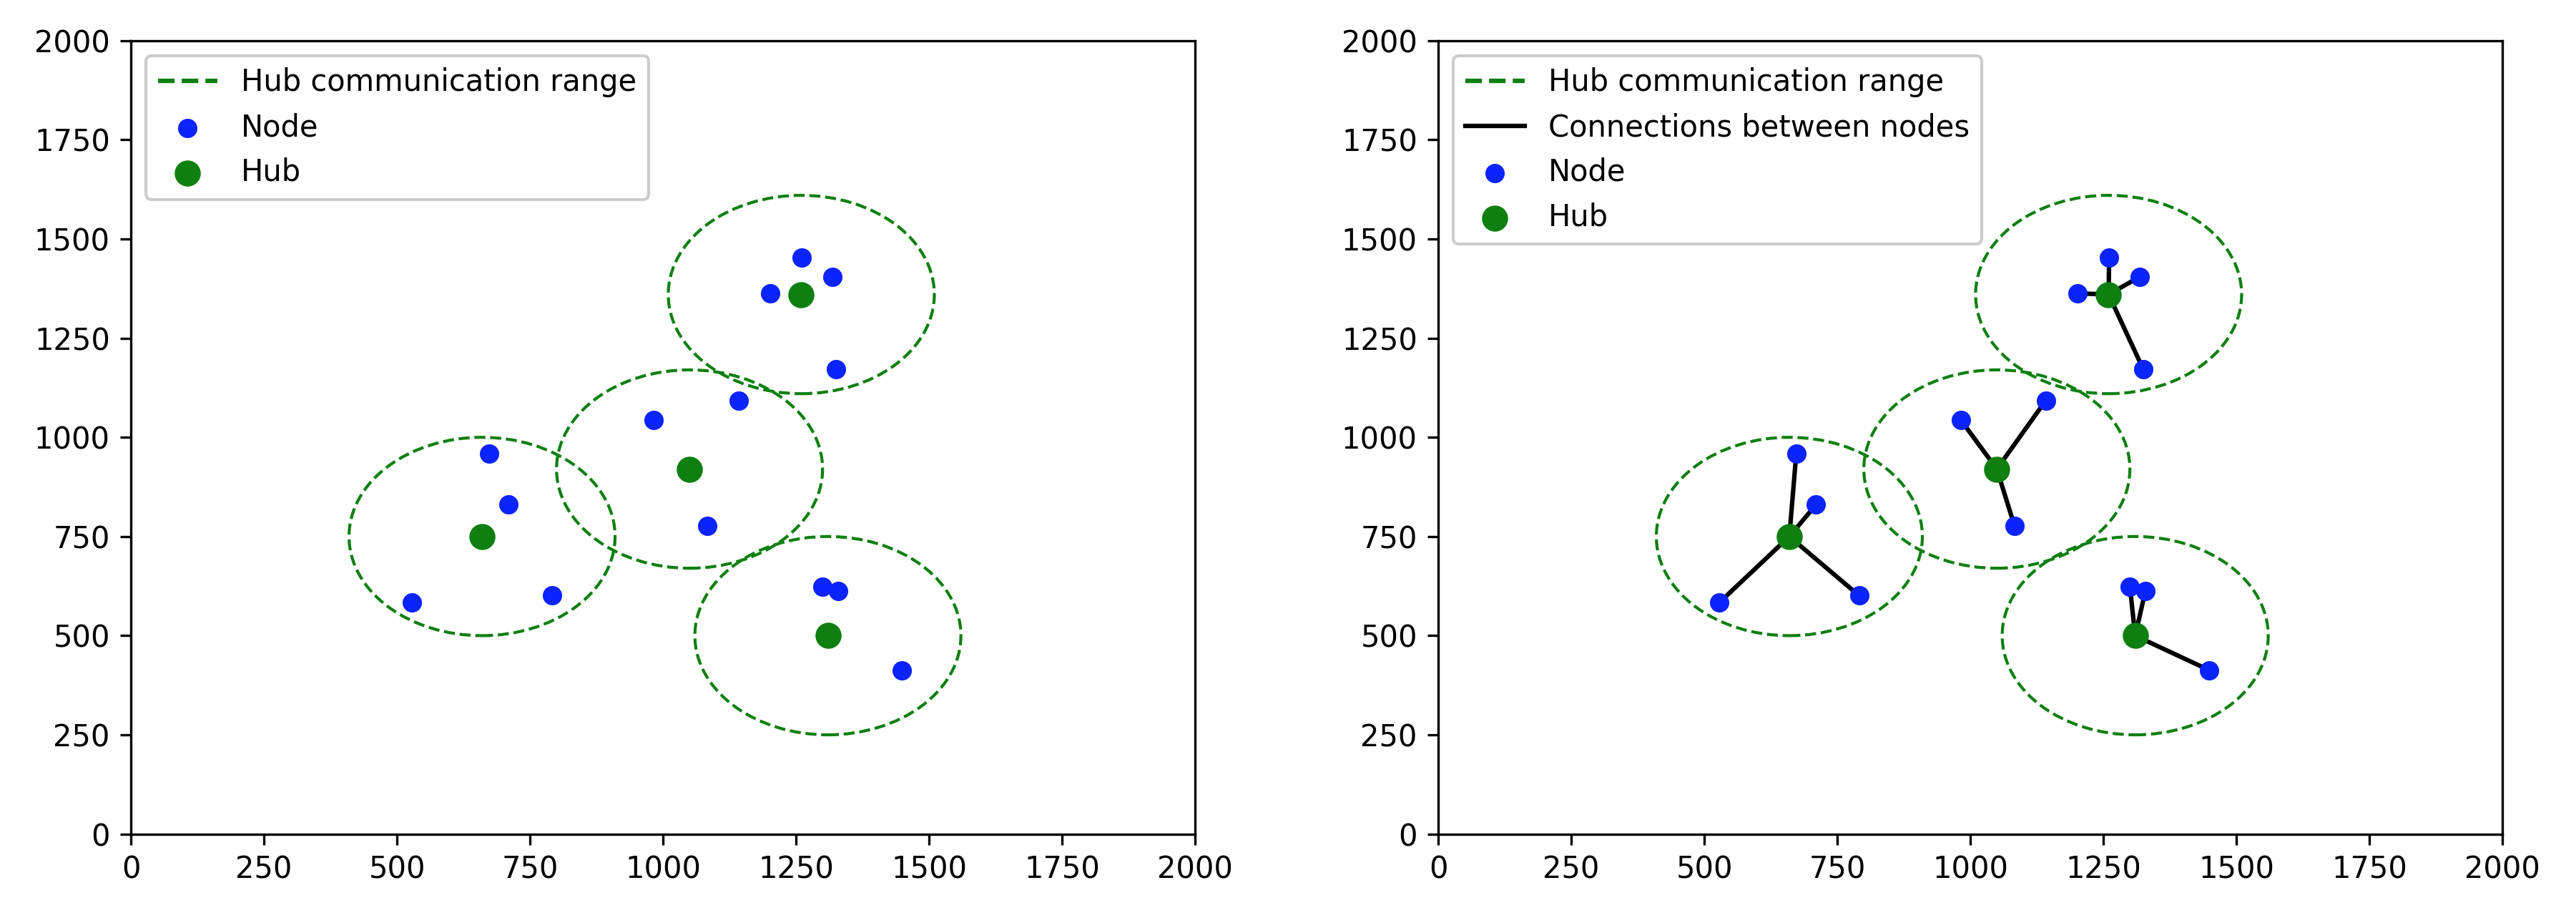
\includegraphics[width=0.94\columnwidth]{final-proposal/images/modeling_star.png}
    \caption{Left: Grouped nodes and corresponding hubs, Right: Nodes connected in hub-spoke (star) network topology based on the communication ranges}
    \label{fig:modeling_star}
\end{figure}

Figure \ref{fig:modeling_complex} demonstrates that the node placement process can be repeated with a greater number of nodes, different communication ranges \& budgets to create more complex hub-spoke and mesh networks
\begin{figure}[H]
    \centering
    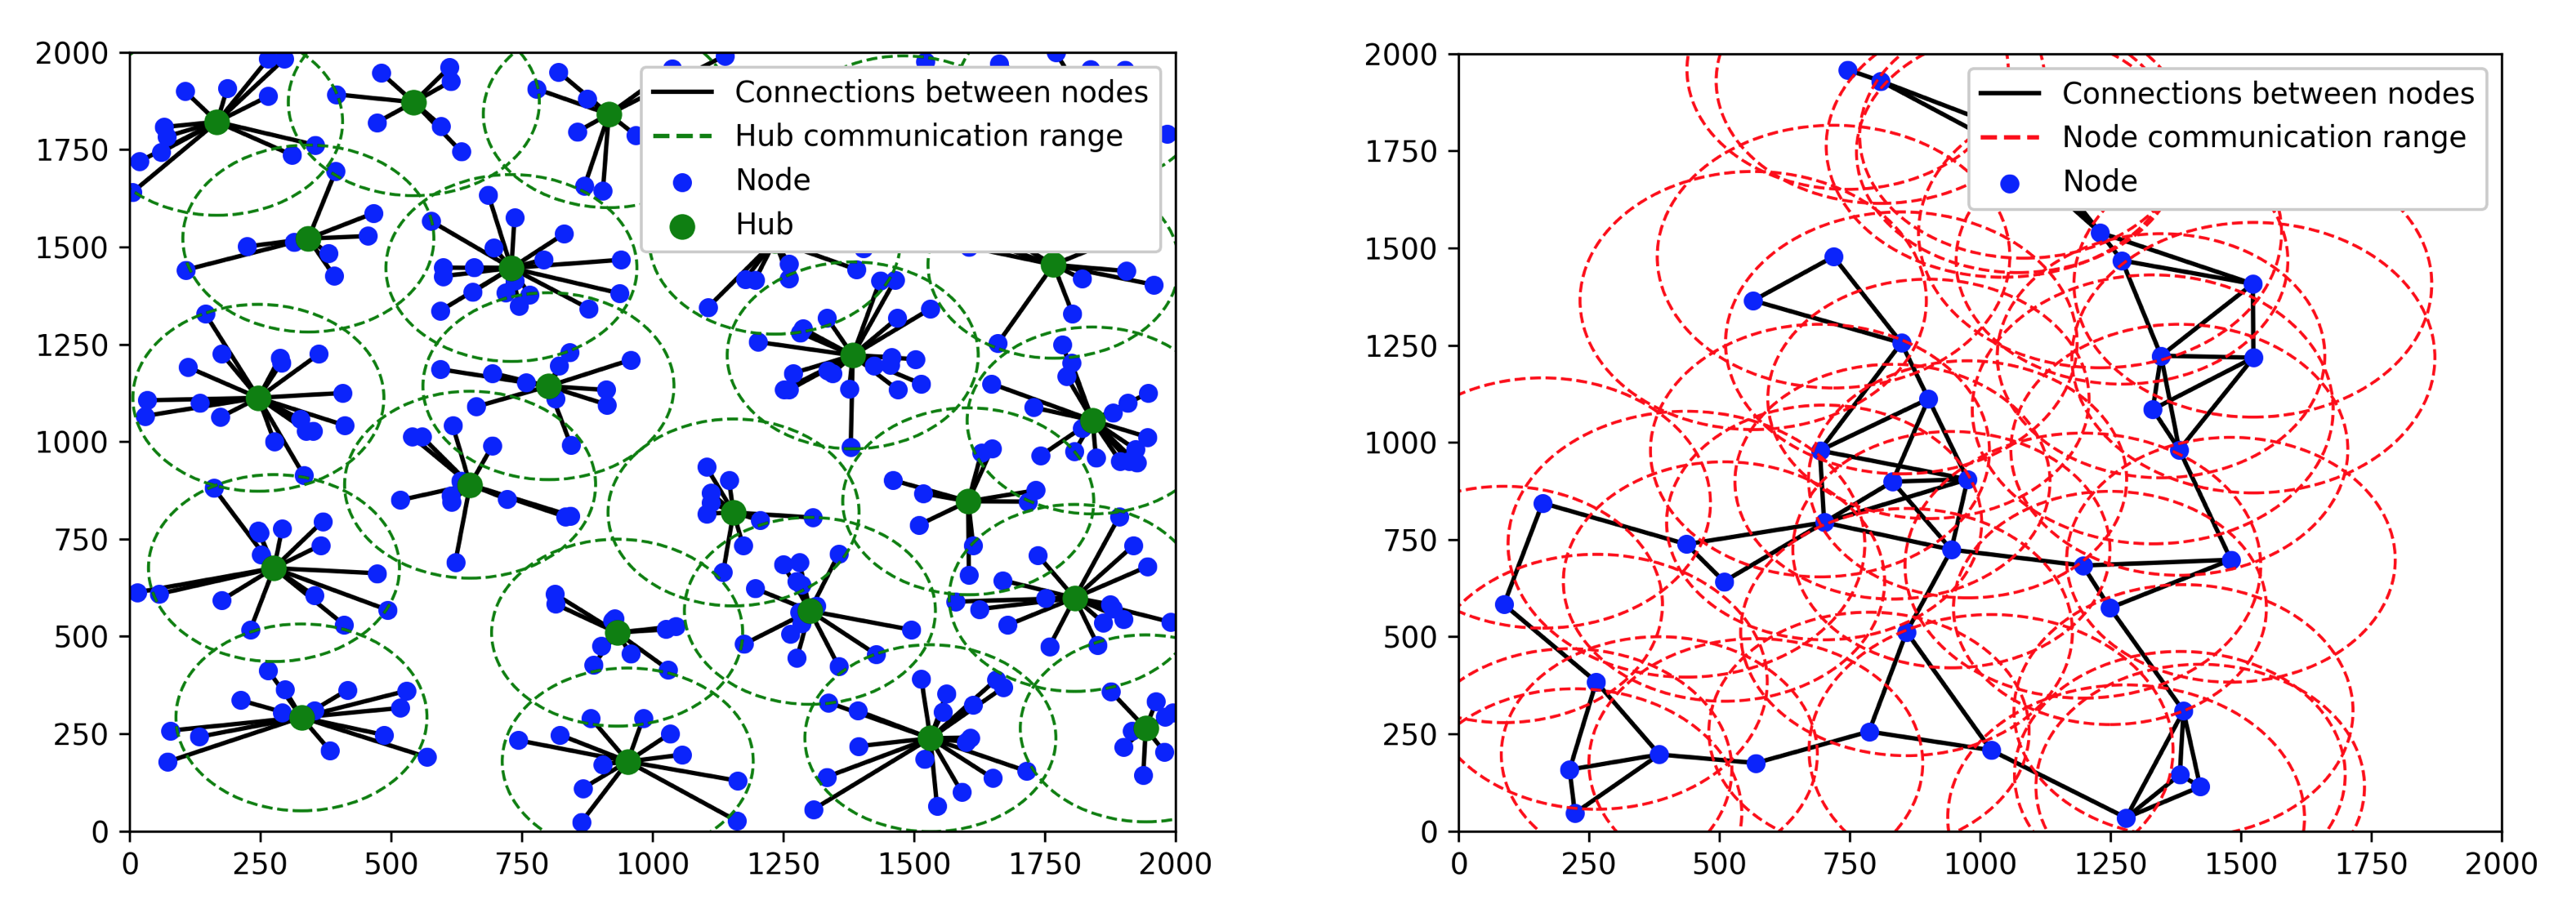
\includegraphics[width=0.94\columnwidth]{final-proposal/images/modeling_complex_unified.png}
    \caption{Left: Hub-spoke (star) network topology created in the virtual space, Right: Mesh network topology created in the virtual space}
    \label{fig:modeling_complex}
\end{figure}

Once the models with desired parameters were constructed using the method outlined above, these models were prepared for network simulations. Thus, the constructed models and the relations between the nodes \& hubs in these models were exported for network communication simulations.

% talk about using python script to output x, y, z parameters (refer to it as \cc{network_generator} script)



%%%%%%%%%%%%%%%%%%%%%%%%%%%%%%%%%%%%%%%%%%
\subsection{Simulation}
We have identified Coracle \cite{Coracle} as a tool to simulate the Raft consensus algorithm on heterogeneous networks. Coracle is a simulation framework written in OCaml programming language, designed to evaluate "distributed consensus algorithms in settings that more accurately represent realistic deployments" \cite{howardCoracleEvaluatingConsensus2015}. The framework allows users to configure nodes, links, and events. 

A node can be defined as a hub, server, client. From experimentation with the framework, we have learned that in the case of a server node, the node acts as a participant and carries out the responsibilities of a typical node, such as voting and log replication. When a node is configured as a hub, it foregoes its responsibility as a participant and acts as a router in the network. Finally, a client node is responsible for generating network traffic within the network between other clients \cite{howardCoracleEvaluatingConsensus2015}.

Links can either be unidirectional or bidirectional; moreover, multiple links between two nodes can exist. Essentially, this allows for the freedom to simulate whether a pair of nodes have half-duplex or full-duplex communication. Furthermore, each link can be assigned a latency category, small, medium, or large, to affect the package delivery time from source to destination nodes. Since we modeled our nodes in a virtual space, we can assign link latency categories based on distances between a pair of connected nodes \cite{howardCoracleEvaluatingConsensus2015}.

Events allow for nodes and links to activate or deactivate at user-defined timestamps. This can simulate unstable networks with multiple unreliable links that periodically fail. Moreover, considering real-world networks, this parameter can also be used to simulate the addition of new nodes into the network, with the only limitation being that node links would be predetermined \cite{howardCoracleEvaluatingConsensus2015}. 

A limitation in modeling and simulation workflow is the lack of traveling nodes, which rebuild their links based on available nearby nodes. We expect to account for this limitation in our physical implementation of the project, where we will be able to test how Raft on mesh behaves with dynamic nodes.

Coracle accepts a JavaScript Object Notation (JSON) file with a specific structure as an input. We expect to write a \cc{simulation\_configuration} script to process the generated network models described in Section \ref{model-gen-section} and generate a JSON file for Coracle. Finally, we expect to write \cc{run\_coracle} script to feed the JSON file into Coracle, run multiple simulations, generate statistics, and display the results. 

For our project, we will generate model networks with 20, 50, 100, 200, 500, and 1000 nodes in areas of 500$m^2$, 1000$m^2$, and 2000$m^2$, for both star and mesh topologies. For each combination, we will run 1000 simulations and gather and study the generated statistics.



%%%%%%%%%%%%%%%%%%%%%%%%%%%%%%%%%%%%%%%%%%
\vspace{-5pt}
\subsection{Experimental Plan}

The experimental plan for our project is as follows:
\begin{enumerate}
    \item Using NetworkX and SciKits software libraries, generate models for star and mesh network topologies in virtual spaces.
    \item Run Coracle simulations on the network models, adjusting for different parameters such as range, maximum distance between nodes, maximum concurrent connections, virtual space, election timeouts, heartbeat intervals, and link failure rate.
    \item Identify and decide upon a mesh communication development kit on ESP8266 chips that can be reasonably modified.
    \item Identify an existing Raft implementation that is suitable for adaptation to operate on our choice of a mesh network. Otherwise, implement Raft ourselves based on previous work and literature.
    \item Test our software library on existing ESP8266 development boards and iterate to obtain satisfactory results.
    \item Run experiments using our software library to compare our real-world results to simulation results.
    \item Design and manufacture a test-bed PCB to fully demonstrate the capabilities of our software library.
\end{enumerate}

The modeling and simulation will help inform the design choices made when implementing the software library. Our design choices of the real-world system will be guided by tweaking simulation parameters to obtain optimal simulation results.

We define the resilience of a network by three parameters: packet delivery rate, average communication latency, and time to leader election. In using the simulations, our efforts will focus on optimizing the system to maximize packet delivery and minimize latency and time to the election. As a result, we will gain an understanding of the range of environments in which our physical system will have effective use.

We will aim to find the conditions under which packet delivery rate is at least 95\%, average latency is at most 20 ms, and time to leader selection is at most 1000ms.
